\documentclass[11pt]{article}

\usepackage[spanish]{babel}
\usepackage{translations}
\usepackage[titles]{tocloft}
\usepackage{multicol}
\usepackage{graphicx}
\usepackage{amsmath}
\usepackage{hyperref}
\usepackage{amsmath}
\usepackage{amssymb}
\usepackage{listings}
\usepackage{courier}
\usepackage[margin=1in]{geometry}
\usepackage{changepage}
\usepackage{titlesec}
\usepackage{wrapfig}
\usepackage[version=4]{mhchem}
\usepackage{multirow}
\usepackage{siunitx}
\usepackage{ragged2e}
\usepackage{adjustbox}
\usepackage[font=small,labelfont=bf]{caption}
\usepackage[table,xcdraw]{xcolor}
\usepackage{afterpage}
\usepackage{xfrac}
\usepackage{animate}
\usepackage{subcaption}
\usepackage{tcolorbox}
\usepackage{nicefrac}

\setlength{\parindent}{1cm}

\definecolor{mytheoremfr}{HTML}{7B0000}
\definecolor{mytheorembg}{HTML}{f5e4e1}

\tcbuselibrary{theorems,skins,hooks}
\newtcbtheorem[number format=\alph]{Theorem}{Pregunta}
{%
	enhanced,
	colback = mytheorembg,
	frame hidden,
	boxrule = 0sp,
	borderline west = {2pt}{0pt}{mytheoremfr},
	sharp corners,
	detach title,
	before upper = \tcbtitle,
	coltitle = mytheoremfr,
	fonttitle = \bfseries\sffamily,
	description font = \mdseries,
	separator sign none,
	segmentation style={solid, mytheoremfr},
}
{th}

\usetikzlibrary{arrows,calc,shadows.blur}
\tcbuselibrary{skins}
\newtcolorbox{note}[1][]{%
	enhanced jigsaw,
	colback=gray!10!white,%
	colframe=gray!80!black,
	size=small,
	boxrule=1pt,
	title=\textbf{Ejercicio:},
	halign title=flush center,
	coltitle=black,
	drop shadow=black!50!white,
	attach boxed title to top left={xshift=1cm,yshift=-\tcboxedtitleheight/2,yshifttext=-\tcboxedtitleheight/2},
	minipage boxed title=2.5cm,
	boxed title style={%
			colback=white,
			size=fbox,
			boxrule=1pt,
			boxsep=2pt,
			underlay={%
					\coordinate (dotA) at ($(interior.west) + (-0.5pt,0)$);
					\coordinate (dotB) at ($(interior.east) + (0.5pt,0)$);
					\begin{scope}[gray!80!black]
						\fill (dotA) circle (2pt);
						\fill (dotB) circle (2pt);
					\end{scope}
				},
		},
	#1,
}

\newcommand{\preguntaAlaMadreDeRocio}[1]{\begin{Theorem}{#1}{}\end{Theorem}}
\newcommand{\laputa}[1]{\begin{note}{#1}{}\end{note}}

\renewcommand{\labelenumi}{\alph{enumi}.}
   
\newcommand{\titulo}{Efecto del Teorema\\ de la Raqueta de Tenis:\\
Efecto Dzhanibekov\\\ \\(Práctica 3)}
\newcommand{\nombreestudiante}{Víctor Mira Ramírez}
\newcommand{\nombredirector}{Luis Antón Ruiz}
\newcommand{\fecha}{\date{Enero 2024}}

\pagebreak

\renewcommand{\listtablename}{Índice de tablas} 
\renewcommand{\tablename}{Tabla} 
\renewcommand\cftsecdotsep{\cftdotsep}

\setlength{\cftbeforesecskip}{0.5ex}
\renewcommand{\cftsecfont}{%
  \fontsize{11}{13}\usefont{OT1}{phv}{bc}{n}\selectfont
}
\makeatletter
\renewcommand{\@pnumwidth}{1.75em}
\renewcommand{\@tocrmarg}{2.75em}
\makeatother

\begin{document}
    \begin{titlepage}
    	\centering
    	
\includegraphics[width=65mm]{fotos/logoUA.png}\par
    	\vspace{1cm}
    	{\huge\bfseries \vspace{15mm} \titulo \par}
    	\vfill
    	{\large 
    	\vfill
    	Estudiante:\par\vspace{2mm}
    	\nombreestudiante\par
    	\vfill
    	Profesor:\par\vspace{2mm}
        \nombredirector
        \vfill
        Universidad de Alicante\par
        Facultad de Ciencias: Departamento de Física Aplicada\par
        Mecánica Newtoniana y Relatividad\par
    	\fecha\par}
    \end{titlepage}
    
    \clearpage

    \begin{abstract}\label{sec:abstract}
		%
	\end{abstract}\vspace{0.3cm}  
    
    \tableofcontents
    \clearpage
        
    \section{Cuestiones propuestas}
        \subsection{Ejes mayor y menor}
            \laputa{Comprueba en los casos estables si las variaciones de las componentes angulares no principales cumplen el comportamiento armónico predicho. Es decir, que sus oscilaciones tienen una frecuencia angular que para el primer eje será:
            \[\omega_{p_1}=\sqrt{\dfrac{(I_1-I_2)(I_1-I_3)}{I_2\ I_3}}\omega_1\]}   
                \vspace{0.1cm}
            \begin{wrapfigure}[13]{r}{0.52\textwidth}
                \vspace{-0.5cm}
                \centering
                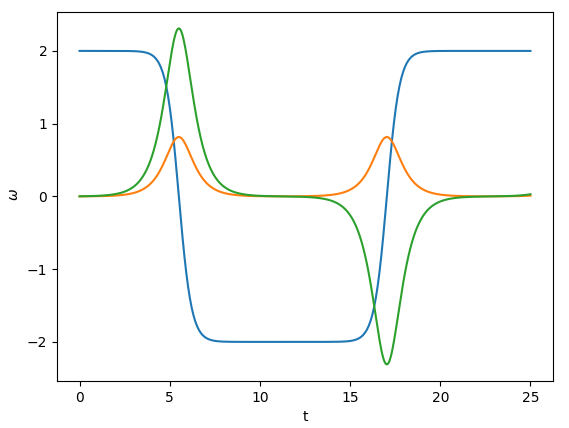
\includegraphics[width=0.5\textwidth]{fotos/graficas/periodo.png}
            \end{wrapfigure}
            
            \noindent Vamos a analizar el programa para comprender cómo calcula el periodo. Observamos cómo para dicho cálculo, es programa busca el máximo y el mínimo de la oscilación en el intervalo de tiempo, midiendo el tiempo que tarda entre ambos puntos. Dicho tiempo es la mitad de una oscilación, por lo que basta multiplicar por dos para obtener el periodo.\\

			\noindent El programa nos da el valor de esta diferencia multiplicada por dos, pero también podemos calcularlo usando la gáfica y el hecho de que los picos están en $t=5.5s$ y $t=17$.
			\[T_\text{consola}=23.046\ s \hspace{1cm}T_\text{gráfico}=23\ s\]

            \noindent Analíticamente, usando la fórmula del enunciado obtenemos que el periodo es 

			\[\omega=\dfrac{2\pi}{T}\Longleftrightarrow T=\dfrac{2\pi}{\omega_{p_1}}\Longleftrightarrow T=\dfrac{2\pi}{\sqrt{\dfrac{(I_1-I_2)(I_1-I_3)}{I_2I_3}}}\omega_1=\dfrac{2\pi}{\sqrt{\dfrac{(4-2)(4-1)}{2\cdot 1}}}\cdot 2=\]

            \clearpage
            \laputa{Comprueba que la energía cinética y que el módulo del momento angular se conservan en este caso. \textit{No hace falta comprobar la precesión}}
				\noindent Basta aplicar las ecuaciones:
				\[E_k=\dfrac12\left(I_1\omega_1^2+I_2\omega_2^2+I_3\omega_3^2\right)\]
				\[L=\sqrt{(I_1\omega_1)^2+(I_2\omega_2)^2+(I_3\omega_3)^2}\]

				\noindent Vemos como tanto la energía cinética como el momento angular se mantienen constantes, pues fijándonos en la escala del gráfico que nos da \textit{matplotlib} vemos que estamos trabajando en el rango de $10^{-5}$, donde la forma de las gráficas se debe al error numérico.\\
				\begin{figure}[h]
					\vspace{-0.2cm}
					\centering
					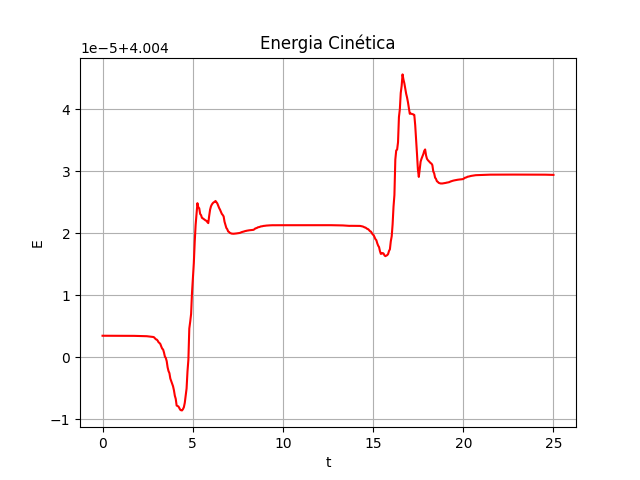
\includegraphics[width=0.49\textwidth]{fotos/graficas/cinetica.png}
					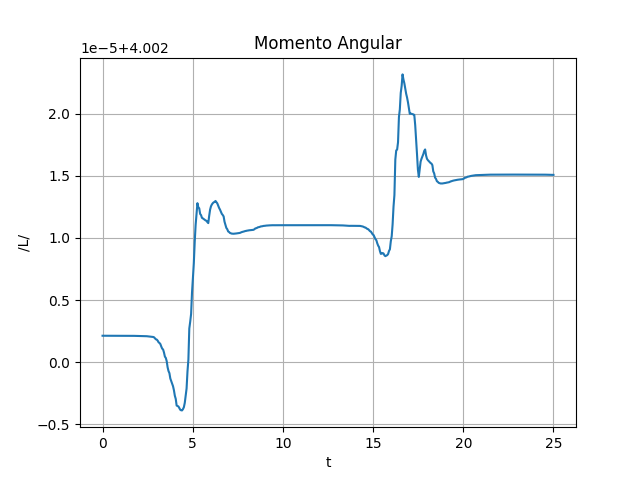
\includegraphics[width=0.49\textwidth]{fotos/graficas/momento_angular.png}
				\end{figure}

				\noindent Si nos ponemos la escala en $10^1$ obtenemos las siguientes gráficas mucho más fáciles de leer.
				\begin{figure}[h]
					\vspace{-0.3cm}
					\centering
					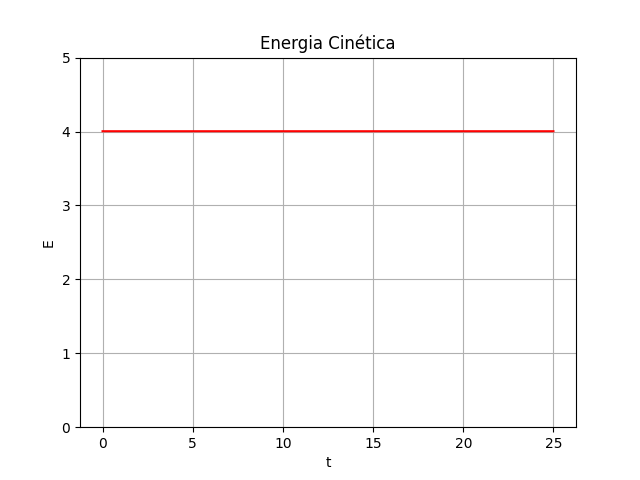
\includegraphics[width=0.49\textwidth]{fotos/graficas/cinetica_escalado.png}
					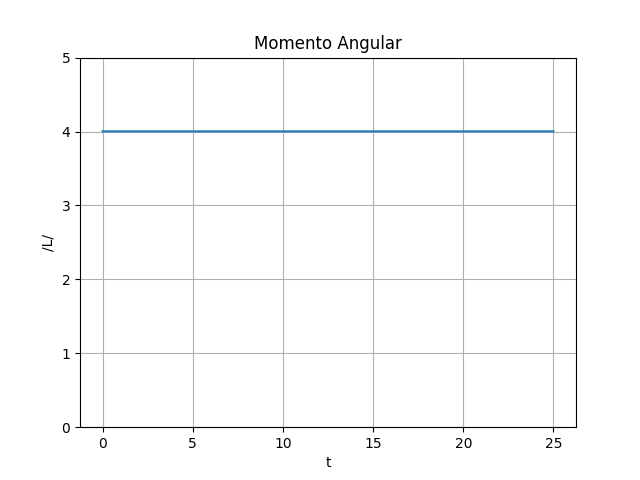
\includegraphics[width=0.49\textwidth]{fotos/graficas/momento_angular_escalado.png}
				\end{figure}

				\noindent Esta variación es la misma para los ejes 1 y 3.
			\clearpage
			\laputa{Comprueba cuál es la evolución del vector velocidad angular y momento angular} % nueva 23-24
				
        \subsection{Eje intermedio}
            \laputa{Comprueba en el caso del eje intermedio cuál es el comportamiento de las componentes de las velocidades angulares. ¿Es periódico el proceso o caótico? En el caso que sea periódico intenta estimar el valor del periodo para un caso e intenta ver qué dependencia parece tener con $\omega_2$}
            \laputa{Representa las componentes $\omega_1$ frente a $\omega_3$, ¿Qué se observa?}
				\begin{wrapfigure}[8]{r}{0.55\textwidth}
					\vspace{-0.65cm}
					\centering
					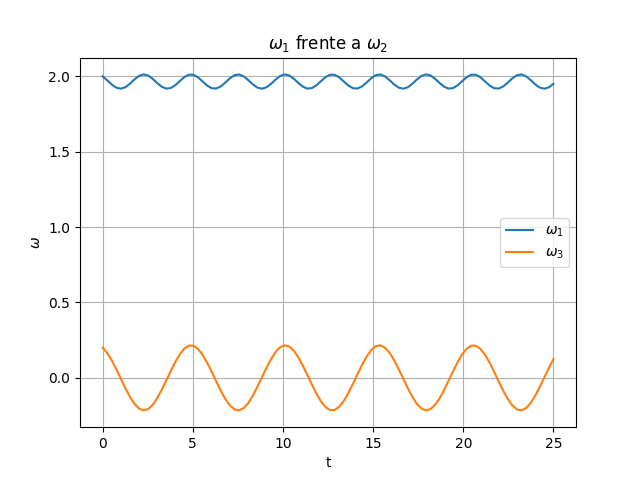
\includegraphics[width=0.54\textwidth]{fotos/graficas/w1frentew2.png}
				\end{wrapfigure}

				\hspace{0cm}\\\hspace{0cm}\\\hspace{0cm}\\\hspace{0cm}\\\noindent En la figura de al lado podemos ver como esta vez nos hallamos en el eje intermedio. Además, notamos que el comportamiento de la velocidad angular de tanto $\omega_1$ como de $\omega_2$ es también armónico.\\
			
			\hspace{0cm}\\\hspace{0cm}\\
            \laputa{Comprueba que la energía cinética y que el módulo del momento angular se conservan en el caso del eje intermedio.}
				\noindent De igual manera que en el eje 1 y 3 obtenemos una gráfica que representa la conservación del módulo del momento angular y de la energía cinética en la escala de $10^1$.
				\begin{figure}[h]
					\vspace{-0.3cm}
					\centering
					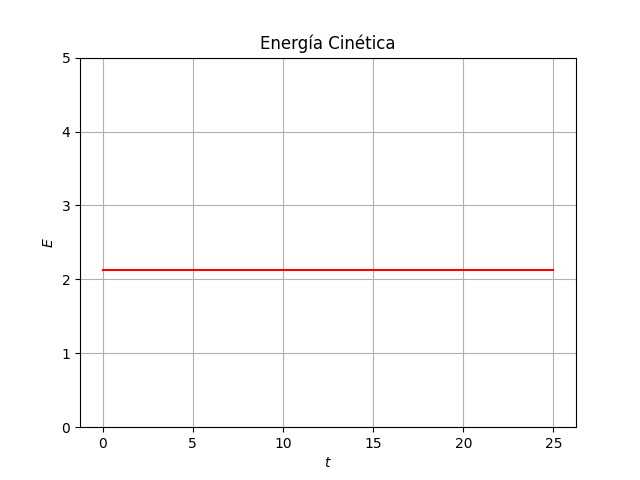
\includegraphics[width=0.49\textwidth]{fotos/graficas/cinetica_intermedio.png}
					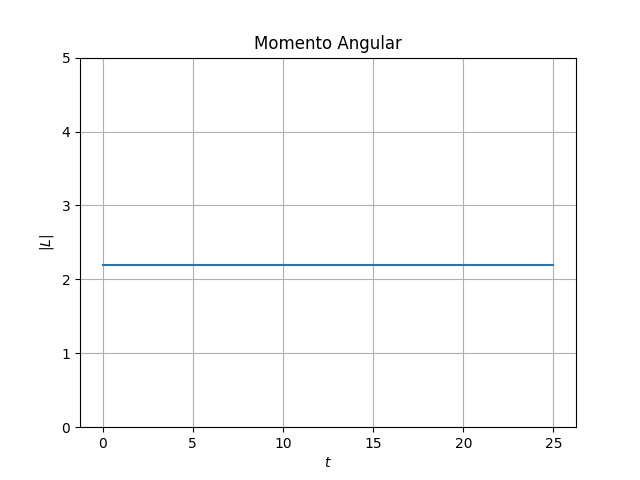
\includegraphics[width=0.49\textwidth]{fotos/graficas/momento_angular_intermedio.png}
				\end{figure}
            \laputa{Dibuja la trayectoria del vector velocidad angular $\vec{\omega}$ y $\vec{L}$. \textit{No hace falta estimar el valor del periodo}}
            \laputa{Razona: Siempre se ha definido que la Tierra es una esfera achatada por los polos. Por lo que tendría dos ejes de simetría iguales y no se aplicaría el teorema. Pero, si no fuera exactamente así, ¿nos deberíamos preocupar por una posible inversión de la rotación del planeta? \textit{No hace falta programar nada, solo explicarlo.}}
            
			\noindent La cuestión nos pregunta qué pasaría si La Tierra fuera una esfera y no una esfera achatada con dos ejes de simetría iguales. Por tanto esta pudiera verse afectada por el \textit{Teorema del Eje Intermedio}.\\
			
			\noindent Sin embargo, sabemos que La Tierra rota respecto a su eje con mayor momento de inercia y no sobre su eje intermedio. Y esto sucede ya que en el caso planteado La Tierra es una esfera siendo por tanto simétrica respecto a sus tres ejes. Es por esto que el \textit{Efecto de la Raqueta de Tenis} no sucedería.\\
                                    
			\noindent Experimentalmente sabemomos que los objetos esféricos llenos de un líquido no rotan especto a su eje intermedio, si no que respecto al eje con mayor momento de inercia. Esto se debe a que por contener líquido su energía cinética no es constante. El cuerpo girará respecto a su eje con menor gasto energético, es decir respecto al que tiene mayor momento de inercia.\\
            
            \noindent La Tierra contiene agua y por ello su energía cinética no es constante. El eje con mayor momento de inercia es el tercero, es decir, La Tierra no rotaría respecto a su eje intermedio y por tanto no sería posible una inversión de la rotación de la misma.\\
    \section{Anexos}
        \subsubsection*{Código de LaTeX que genera este documento:}
            \href{https://www.overleaf.com/read/ghsbdxtsnhtj#09bdf3}{MECN-Practica1:raqueta.tex}

\end{document} 